\documentclass[]{article}
\usepackage{graphicx}
%opening
\title{Appunti di Automi e Linguaggi Formali}
\author{Nicola Baesso}

\begin{document}

\maketitle

\newpage
\tableofcontents
\newpage

\textbf{Disclaimer}
\newline
\newline
Questi appunti sono una raccolta parziale delle spiegazioni del prof. Bresolin, e sono state scritte con la gioia di poterle portare al primo parziale dell'anno. Si consiglia comunque di utilizzare solo come eventuale ripasso e non come testo di studio.
\newpage
\section{Introduzione}
\subsection{Definizioni utili alla comprensione}
Per questo corso, ci si avvarrà di alcune definizioni riportate in seguito, utili per una migliore comprensione della materia.
\subsubsection{Algoritmi e Problemi}
Un problema è definito da 3 (tre) caratteristiche specifiche: l'insieme dei possibili input, l'insieme dei possibili output e la relazione che collega questi due insiemi.
\newline
Un algoritmo è una procedura meccanica che, eseguendo delle computazioni eseguibili da un calcolatore, risolve un determinato problema se per ogni input si ferma dopo un numero finito di passaggi e produce un output corretto.
\newline Inoltre è composto da una complessità temporale, che indica il tempo di esecuzione, e una complessità spaziale, che indica la quantità di memoria utilizzata. Entrambe queste misure sono dipendenti dalla dimensione dell'input.
\subsubsection{Linguaggi formali}
Un linguaggio formale può essere definito come un'astrazione del concetto di problema. 
\newline
Infatti, un problema può essere espresso sia come un insieme di stringhe (che da qui in avanti indicheremo con Linguaggio), con soluzioni che indicano se una stringa è presente nel Linguaggio o meno, oppure come una trasformazione tra vari Linguaggi, dove la soluzione trasforma una stringa di input in una stringa di output.
\newline
Quindi, ogni processo computazionale può essere ridotto ad una determinazione dell'appartenenza ad un insieme di stringhe, oppure essere ridotto ad una mappatura tra insiemi di stringhe.
\subsubsection{Automi}
Un automa è un dispositivo matematico (inteso in forma astratta) che può determinare l'appartenenza di una stringa ad un Linguaggio e può trasformare una stringa in una seconda stringa. Possiede ogni aspetto di un computer, poichè dato un input provvede a fornire un output, è dotato di memoria e ha la capacità di prendere delle decisioni.
\newline
La memoria per un automa è fondamentale. Sostanzialmente esistono automi a memoria finita e automi a memoria infinita, quest'ultimi con accesso limitato e non.
\newline Chiaramente si hanno vari tipi di automi, ognuno di questi adatti ad una determinata classe di linguaggi, dove vengono differenziati per quantità di memoria e per il tipo di accesso ad essa.
\subsubsection{Alfabeto e Linguaggio}
Esattamente come nel caso del linguaggio naturale, un alfabeto è un insieme finito e non vuoto di simboli, ed è indicato con il simbolo $\Sigma$. Da esso si ha la stringa, ovvero una sequenza finita di simboli presi da un alfabeto. Inoltre, si definisce come stringa vuota la stringa senza alcun simbolo preso dall'alfabeto, e si indica con il simbolo $\varepsilon$. Infine la lunghezza di una stringa indica il numero di simboli presenti nella stringa, indicandola con \textbar w\textbar, con w una stringa qualsiasi .
\newline
\newline
\textbf{Esempio}
Si consideri il codice binario, composto da 0 ed 1. Allora definiremo l'alfabeto come $\Sigma$=\{0,1\}, una stringa valida come w=010110, e in questo particolare caso \textbar w\textbar=6.
\newline
\newline
La potenza di un alfabeto, espressa come $\Sigma$$^k$ con k$\textgreater$0, esprime l'insieme delle stringhe composte da simboli dell'alfabeto di lunghezza k. L'espressione $\Sigma$$^*$ indica l'insieme di tutte le stringhe sull'alfabeto.
\newline
\newline
\textbf{Esempio}
Consideriamo nuovamente il codice binario. Per 0$\textless$k$\textless$2 (inclusi) si ha \newline
$\Sigma$$^0$=$\varepsilon$ (la stringa vuota) \newline
$\Sigma$$^1$=\{0,1\}\newline
$\Sigma$$^2$=\{00,01,10,11\} \newline
E così per ogni k positivo. Mentre $\Sigma$$^*$=$\Sigma$$^0$ $\cup$ $\Sigma$$^1$ $\cup$ $\Sigma$$^2$ \ldots \newline \newline 
Quindi la potenza di un alfabeto crea a sua volta un alfabeto, con stringhe di lunghezza k, e tale alfabeto è composto da 2$^k$ stringhe. 
\newline
\newline
Un linguaggio L è un sottoinsieme dell'insieme di tutte le stringhe dell'alfabeto. In simboli: L $\subseteq$ $\Sigma$$^*$ per un certo $\Sigma$.
\section{DFA, NFA, espressioni e Linguaggi (non) regolari}
\subsection{DFA}
Gli Automi a Stati Finiti (in Inglese Deterministic Finite Automation, abbreviato in DFA) sono la forma più semplice di automa e dispongono di una quantità finita di memoria.
Tali automi accettano una parola nel linguaggio unicamente se è in uno stato terminale.
\newline
\newline
\textbf{Esempio}
Trovare ogni parola nel linguaggio binario che sia composta da un numero pari di 1.\newline
Per creare questro DFA, abbiamo bisogno di due stati:\newline
-Il primo sarà lo stato con il numero pari di 1. Tale stato sarà sia iniziale che terminale (e quindi accetterà la stringa).\newline
-Il secondo sarà lo stato nel quale si ha un numero dispari di 1. In tale stato l'automa non accetterà la stringa.\newline
Nel caso s'incontri uno 0, si deve rimanere nello stato attuale.\newline
Segue immagine dell'automa, fatta su JFlap:
\newline
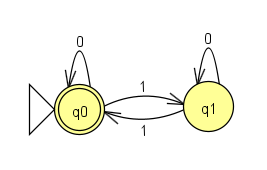
\includegraphics{DFA1.png}
\newline
\newline
Si noti, nel esempio, che ogni stato esegue una transazione \textbf{per ogni simbolo nel linguaggio}. Inoltre, quello che fa l'automa è semplicemente "contare" quante cifre di 1 sono presenti, accettando la stringa solo quando questa cifra è pari.
\section{Grammatiche di Linguaggi liberi da contesto e PDA}
\end{document}
